\begin{savequote}[8cm]
\begin{CJK*}{UTF8}{gbsn}
  欲说还休,却道天凉好个秋。
\end{CJK*}

Life is ... like ... well ... the weather here.

  \qauthor{--- Qiji Xin \textit{Chou Nu Er}}
\end{savequote}

\chapter{\label{app:tuning}Tuning supplementary plots}

\minitoc

% \section{Combinations of Observables}\label{sec:appcombi}


% Table~\ref{tab:fit-var-combo} displays the tested combinations of observables:
% \begin{itemize}
%     \item \textbf{\texttt{Combi-}1 through 5} are cross-experiment selections of a single observable. 
% For example, \texttt{Combi-}$3$ uses only $\dat$ from all four data sets. If a chosen observable is absent from a dataset, that dataset is excluded from the specific combination. 
% For example, \ttkzpi is not used in \texttt{Combi-}1 due to the absence of $\pn$.
% \item \textbf{\texttt{Combi-}6 through 9} incorporate all variables from a single measurement. For example, \texttt{Combi-}$9$ uses \minpiz only.
% \item \textbf{\texttt{Combi-}10 to 13} uses two out of four measurements according to the experiment or topology. For example, \texttt{Combi-}$10$ uses only the two data sets from T2K, and \texttt{Combi-}$13$  only with pion production. 
% \item \textbf{\texttt{Combi-}14 to 17} combine two separate combinations:
% \begin{align*}
% \texttt{Combi-14} &= \texttt{Combi-3} \cup \texttt{Combi-5},\\
% \texttt{Combi-15} &= \texttt{Combi-1} \cup \texttt{Combi-2},\\
% \texttt{Combi-16} &= \texttt{Combi-1} \cup \texttt{Combi-3},\\
% \texttt{Combi-17} &= \texttt{Combi-2} \cup \texttt{Combi-3}.
% \end{align*}
% \item \textbf{\texttt{Combi-}18 through 22} result from merging three combinations:
% \begin{align*}
% \texttt{Combi-18} &= \texttt{Combi-1} \cup \texttt{Combi-3} \cup \texttt{Combi-5},\\
% \texttt{Combi-19} &= \texttt{Combi-2} \cup \texttt{Combi-3} \cup \texttt{Combi-5},\\
% \texttt{Combi-20} &= \texttt{Combi-3} \cup \texttt{Combi-4} \cup \texttt{Combi-5},\\
% \texttt{Combi-21} &= \texttt{Combi-1} \cup \texttt{Combi-2} \cup \texttt{Combi-3},\\
% \texttt{Combi-22} &= \texttt{Combi-1} \cup \texttt{Combi-2} \cup \texttt{Combi-4}.
% \end{align*}
% \item \textbf{\texttt{Combi-}23} merges four different combinations:
% \begin{align*}
% \texttt{Combi-23} &= \texttt{Combi-1} \cup \texttt{Combi-2} \cup \\
% & \texttt{Combi-3} \cup \texttt{Combi-5}.
% \end{align*}
% \item \textbf{\texttt{Combi-}24} encompasses all variables, acting as the superset.
% \item \textbf{\texttt{Combi-}25 and 26} are the same as \texttt{Combi-}$21$ and $23$, respectively, except that $\dpt$ in \minzpi is removed to avoid correlation with $\pn$ in the same data set.
% \end{itemize}

% Figure~\ref{fig:allchi} shows the change in $\chi^2$ for the complete observable set (tuned plus validation) as a function of the tuning combination, where the two model parameter sets, \allpar and \redpar, are compared and it can be seen that the respective minima happen at \texttt{Combi-15} and 26. 
 

\section*{$\piz$ FSI fate decomposition for \gZero\ and \gC}\label{sec:appfate}

Figures~\ref{fig:g24-0-dat-pi0}-\ref{fig:g24-c-pn-pi0} display comparisons of \gZero\ and \gC\ predictions to data, detailing the composition by $\piz$ FSI fate.

% \newpage

% \begin{table*}[h]
% \begin{tabular}{l|lllll|llll|llll|lp{1cm}ll|lllll|l|p{1cm}|lp{1cm}}
% \hline
% \hline
%  \texttt{Combi-}        & 1 & 2 & 3 & 4 & 5 & 6 & 7 & 8 & 9 & 10 & 11 & 12 & 13 & 14 & 15 \par (\texttt{Best-}\par\allpar) & 16 & 17 & 18 & 19 & 20 & 21 & 22 & 23 & 24 \par (\texttt{Super-}\par\texttt{set}) & 25 & 26 \par (\texttt{Best-}\par\redpar)\\
%          \hline
% \multicolumn{27}{c}{\ttkzpi} \\
% \hline
% $\dat$      &   &   & $\tick$ &   &   & $\tick$ &   &   &   & $\tick$  &    & $\tick$  &    & $\tick$  &    & $\tick$  & $\tick$  & $\tick$  & $\tick$  & $\tick$  & $\tick$  &    & $\tick$  & $\tick$  & $\tick$  & $\tick$  \\
% $\dpt$   &   & $\tick$ &   &   &   & $\tick$ &   &   &   & $\tick$  &    & $\tick$  &    &    & $\tick$  &    & $\tick$  &    & $\tick$  &    & $\tick$  & $\tick$  & $\tick$  & $\tick$  & $\tick$  & $\tick$  \\
% $\dphit$ &   &   &   & $\tick$ &   & $\tick$ &   &   &   & $\tick$  &    & $\tick$  &    &    &    &    &    &    &    & $\tick$  &    & $\tick$  &    & $\tick$  &    &    \\
% \hline
% \multicolumn{27}{c}{\ttkpip} \\
% \hline
% $\dat$      &   &   & $\tick$ &   &   &   & $\tick$ &   &   & $\tick$  &    &    & $\tick$  & $\tick$  &    & $\tick$  & $\tick$  & $\tick$  & $\tick$  & $\tick$  & $\tick$  &    & $\tick$  & $\tick$  & $\tick$  & $\tick$  \\
% $\pn$       & $\tick$ &   &   &   &   &   & $\tick$ &   &   & $\tick$  &    &    & $\tick$  &    & $\tick$  & $\tick$  &    & $\tick$  &    &    & $\tick$  & $\tick$  & $\tick$  & $\tick$  & $\tick$  & $\tick$  \\
% $\dptt$     &   &   &   &   & $\tick$ &   & $\tick$ &   &   & $\tick$  &    &    & $\tick$  & $\tick$  &    &    &    & $\tick$  & $\tick$  & $\tick$  &    &    & $\tick$  & $\tick$  &    & $\tick$  \\
% \hline
% \multicolumn{27}{c}{\minzpi} \\
% \hline
% $\dat$      &   &   & $\tick$ &   &   &   &   & $\tick$ &   &    & $\tick$  & $\tick$  &    & $\tick$  &    & $\tick$  & $\tick$  & $\tick$  & $\tick$  & $\tick$  & $\tick$  &    & $\tick$  & $\tick$  & $\tick$  & $\tick$  \\
% $\pn$       & $\tick$ &   &   &   &   &   &   & $\tick$ &   &    & $\tick$  & $\tick$  &    &    & $\tick$  & $\tick$  &    & $\tick$  &    &    & $\tick$  & $\tick$  & $\tick$  & $\tick$  & $\tick$  & $\tick$  \\
% $\dpt$      &   & $\tick$ &   &   &   &   &   & $\tick$ &   &    & $\tick$  & $\tick$  &    &    & $\tick$  &    & $\tick$  &    & $\tick$  &    & $\tick$  & $\tick$  & $\tick$  & $\tick$  &    &    \\
% $\dphit$    &   &   &   & $\tick$ &   &   &   & $\tick$ &   &    & $\tick$  & $\tick$  &    &    &    &    &    &    &    & $\tick$  &    & $\tick$  &    & $\tick$  &    &    \\
% \hline
% \multicolumn{27}{c}{\minpiz} \\
% \hline
% $\dat$      &   &   & $\tick$ &   &   &   &   &   & $\tick$ &    & $\tick$  &    & $\tick$  & $\tick$  &    & $\tick$  & $\tick$  & $\tick$  & $\tick$  & $\tick$  & $\tick$  &    & $\tick$  & $\tick$  & $\tick$  & $\tick$  \\
% $\pn$       & $\tick$ &   &   &   &   &   &   &   & $\tick$ &    & $\tick$  &    & $\tick$  &    & $\tick$  & $\tick$  &    & $\tick$  &    &    & $\tick$  & $\tick$  & $\tick$  & $\tick$  & $\tick$  & $\tick$  \\
% $\dptt$     &   &   &   &   & $\tick$ &   &   &   & $\tick$ &    & $\tick$  &    & $\tick$  & $\tick$  &    &    &    & $\tick$  & $\tick$  & $\tick$  &    &    & $\tick$  & $\tick$  &    & $\tick$ \\
% \hline
% \hline    
% \end{tabular}
% \caption{\label{tab:fit-var-combo}
% Specifications of observable combinations within the tuning superset in Table~\ref{tab:data-sets}. \texttt{Combi-15} is \texttt{Best-}\allpar, \texttt{Combi-24} is \texttt{Superset}, and \texttt{Combi-26} is \texttt{Best-}\redpar. 
% }
% \end{table*}

\begin{figure*}[!htb] 
\centering 		
    \includegraphics[width=\dbfigwid\textwidth]{figures/tuning/0000-t2k_0pi_dalphat_pi0_decomp.eps} 
    \includegraphics[width=\dbfigwid\textwidth]{figures/tuning/0000-t2k_pip_dalphat_pi0_decomp.eps} 
    \includegraphics[width=\dbfigwid\textwidth]{figures/tuning/0000-min_0pi_dalphat_pi0_decomp.eps} 
    \includegraphics[width=\dbfigwid\textwidth]{figures/tuning/0000-min_pi0_dalphat_pi0_decomp.eps}
    \caption{\label{fig:g24-0-dat-pi0} Extension of figure~\ref{fig:CEX-minpiz-dat-pi0}a to all four $\dat$ measurements. }   		
    \includegraphics[width=\dbfigwid\textwidth]{figures/tuning/0000-t2k_0pi_dpt_pi0_decomp.eps}
    \includegraphics[width=\dbfigwid\textwidth]{figures/tuning/0000-t2k_pip_pn_pi0_decomp.eps}
    \includegraphics[width=\dbfigwid\textwidth]{figures/tuning/0000-min_0pi_pn_pi0_decomp.eps}
    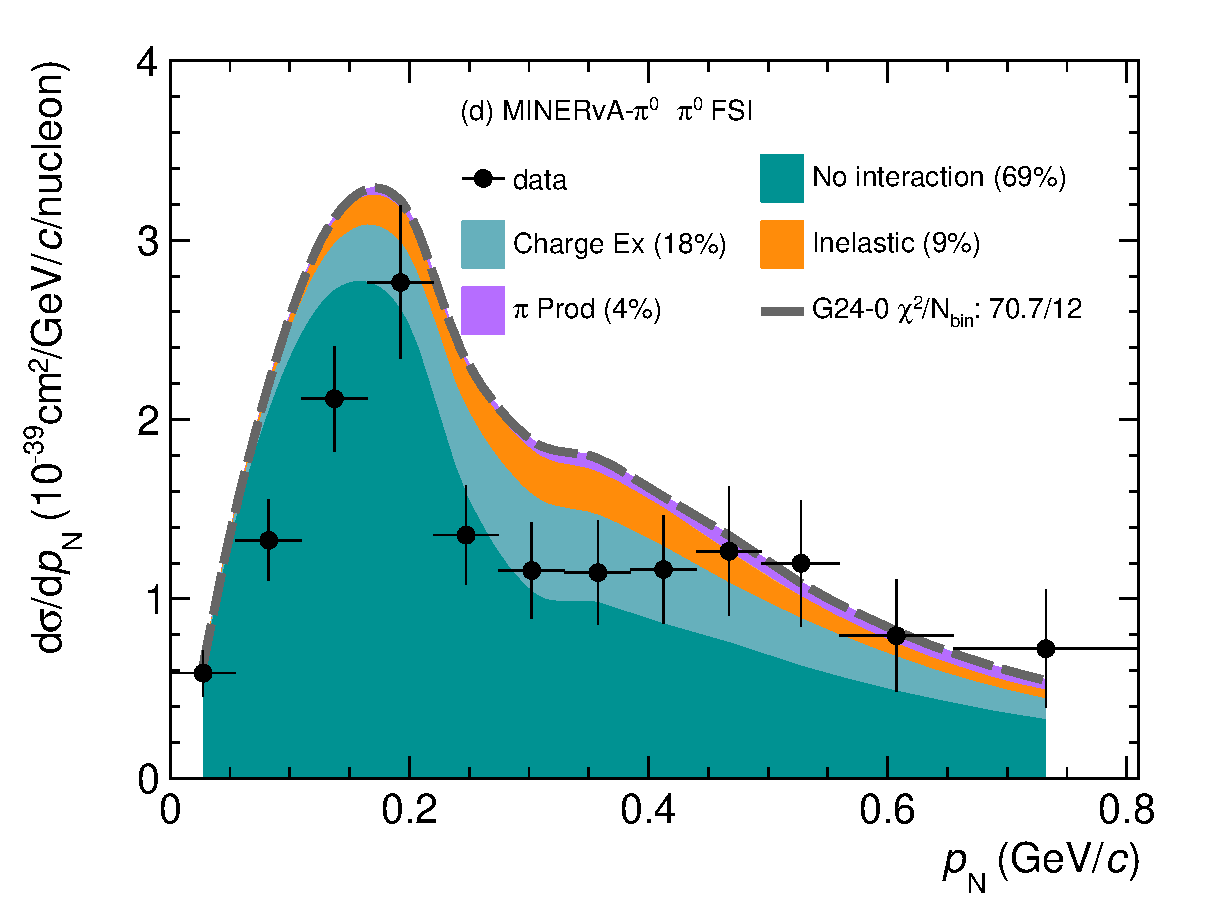
\includegraphics[width=\dbfigwid\textwidth]{figures/tuning/0000-min_pi0_pn_pi0_decomp.eps}
    \caption{\label{fig:g24-0-pn-pi0}  Extension of figure~\ref{fig:CEX-minpiz-dat-pi0}a but to all four $\pn$ measurements. } 
\end{figure*}

\begin{figure*}[!htb] 
    \centering 		
    \includegraphics[width=\dbfigwid\textwidth]{figures/tuning/0026-t2k_0pi_dalphat_pi0_decomp_covfix.eps}
    \includegraphics[width=\dbfigwid\textwidth]{figures/tuning/0026-t2k_pip_dalphat_pi0_decomp_covfix.eps}
    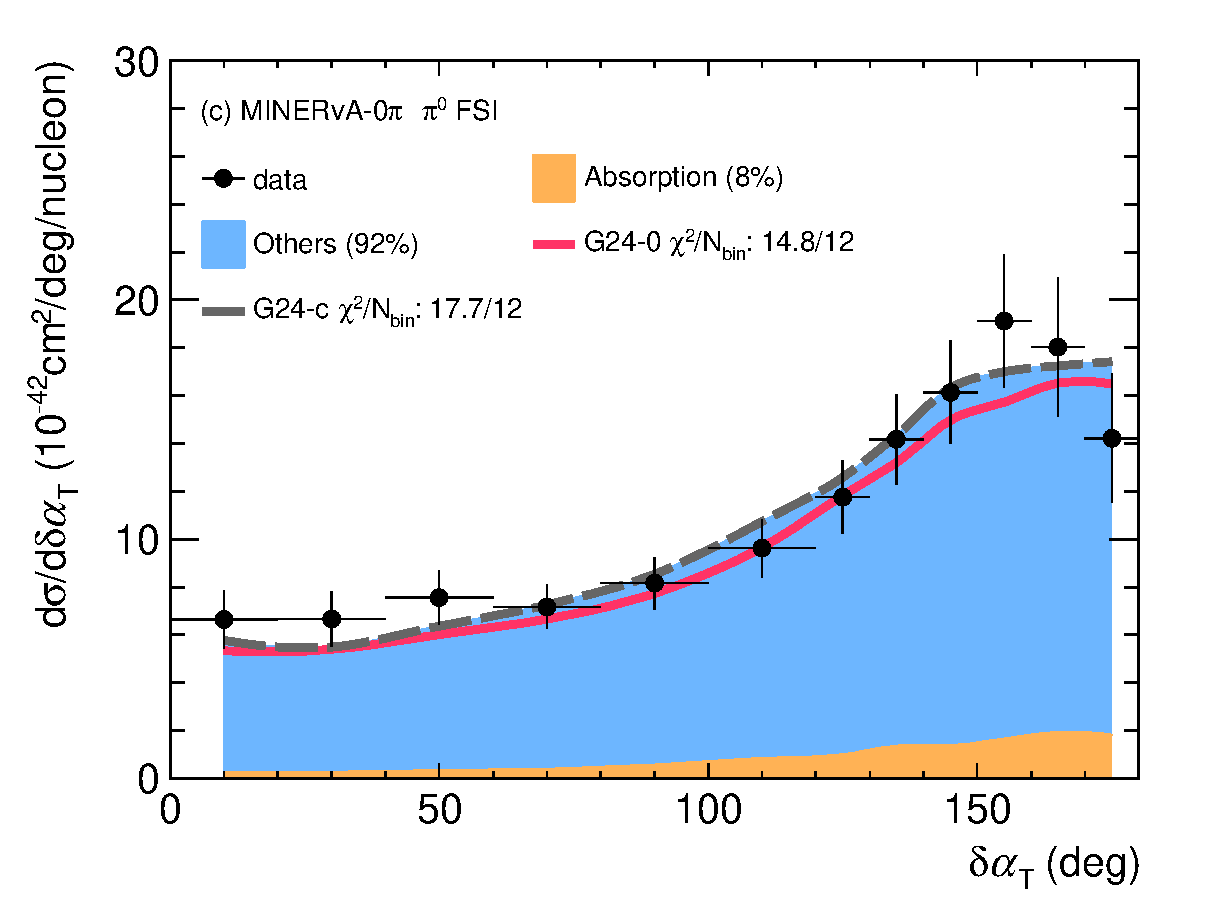
\includegraphics[width=\dbfigwid\textwidth]{figures/tuning/0026-min_0pi_dalphat_pi0_decomp_covfix.eps}
    \includegraphics[width=\dbfigwid\textwidth]{figures/tuning/0026-min_pi0_dalphat_pi0_decomp_covfix.eps}
    \caption{\label{fig:g24-c-dat-pi0} Extension of figure~\ref{fig:CEX-minpiz-dat-pi0}b to all four $\dat$ measurements. } 
		
    \includegraphics[width=\dbfigwid\textwidth]{figures/tuning/0026-t2k_0pi_dpt_pi0_decomp_covfix.eps}
    \includegraphics[width=\dbfigwid\textwidth]{figures/tuning/0026-t2k_pip_pn_pi0_decomp_covfix.eps}	
    \includegraphics[width=\dbfigwid\textwidth]{figures/tuning/0026-min_0pi_pn_pi0_decomp_covfix.eps}
    \includegraphics[width=\dbfigwid\textwidth]{figures/tuning/0026-min_pi0_pn_pi0_decomp_covfix.eps}
    \caption{\label{fig:g24-c-pn-pi0} Extension of figure~\ref{fig:CEX-minpiz-dat-pi0}b but to all four $\pn$ measurements.} 
\end{figure*}

